%%%%%%%%%%%%%%%%%%%%%%%%%%%%%%%%%%%%%%%%%%%%%%%%%%%%%%%%%%%%%%%%%%%%%%
% Universidad de Costa Rica
% Escuela de Ingeniería Eléctrica
% IE0308 - Laboratorio Eléctrico I
% IE0408 - Laboratorio Eléctrico II
%
% FORMATO DE ANTEPROYECTOS Y REPORTES DE LABORATORIO
%
% Elaborado por:
% Fabián Abarca Calderón
%
% Revisado por:
% Diego Dumani Jarquín
% Jaime Cascante Vindas
%
% Última versión:
% Marzo 2016
%%%%%%%%%%%%%%%%%%%%%%%%%%%%%%%%%%%%%%%%%%%%%%%%%%%%%%%%%%%%%%%%%%%%%%





\documentclass[letterpaper,tikz,multi=false,border=5mm]{article}     % Tipo de documento y otras especificaciones
\usepackage{lipsum}
\usepackage{tikz}


\usepackage[utf8]{inputenc}                   % Para escribir tildes y eñes
\usepackage[spanish]{babel}                   % Para que los títulos de figuras, tablas y otros estén en español
\usepackage{lscape}
\addto\captionsspanish{\renewcommand{\tablename}{Tabla}}					% Cambiar nombre a tablas
\addto\captionsspanish{\renewcommand{\listtablename}{Índice de tablas}}		% Cambiar nombre a lista de tablas

\usepackage{ucs}
\usepackage{url}
\usepackage{amsmath}      % Los paquetes ams son desarrollados por la American Mathematical Society
\usepackage{amsfonts}     % y mejoran la escritura de fórmulas y símbolos matemáticos.
\usepackage{amssymb}
\usepackage{graphicx}     % Para insertar gráficas
\usepackage[lofdepth,lotdepth]{subfig}	% Para colocar varias figuras
\usepackage{unitsdef}	  % Para la presentación correcta de unidades

\usepackage[colorlinks=true,urlcolor=blue,linkcolor=black,citecolor=green]{hyperref}     % Para insertar hipervínculos y marcadores
\usepackage{float}		% Para ubicar las tablas y figuras justo después del texto
\usepackage{booktabs}	% Para hacer tablas más estilizadas


\renewcommand{\unitvaluesep}{\hspace*{4pt}}	% Redimensionamiento del espacio entre magnitud y unidad
\batchmode
\usepackage{geometry}
\geometry{left=18mm,right=18mm,top=21mm,bottom=21mm} % Tamaño del área de escritura de la página
\bibliographystyle{plain}
\pagestyle{plain}
\usepackage{pdfpages} % to import PDF pages
\pagenumbering{arabic}
\usepackage{lastpage}
\usepackage{fancyhdr}	% Para manejar los encabezados y pies de página
\pagestyle{fancy}		% Contenido de los encabezados y pies de pagina
\lhead{Química orgánica 2}
\chead{}
\rhead{Cuadro de constantes}
\lfoot{Escuela de Química}
\cfoot{\thepage\ de \pageref{LastPage}}
\rfoot{Universidad de Costa Rica}
\newcommand{\celsiu}{^\circ}
\newcommand{\imagen}[3]{\resizebox{\hsize}{!}{\includegraphics[width=#1mm, height=#2mm]{#3}}}
\newcommand{\toxicologia}[4][1]{\footnotesize{ \begin{tabular}{l}
\begin{tabular}[c]{@{}l@{}}#1\\ #2 \\#3 \\#4\end{tabular}
\end{tabular}}}

\let\OLDthebibliography=\thebibliography
\def\thebibliography#1{\OLDthebibliography{#1}%
\addcontentsline{toc}{section}{\refname}}


\makeatletter
\renewcommand\@biblabel[1]{#1. \ }
\makeatother


%%%%%%%%%%%%%%%%
\begin{document}	% Inicio del documento
%%%%%%%%%%%%%%%%



 % PAGINA 2: RESUMEN %Palabras claves
%%%%%%%%%%%%%%%%ja Fabricante 2N2222}
\begin{landscape}


\begin{table}[]
\begin{tabular}{lllllllll}
\hline
Nombre & \begin{tabular}[c]{@{}l@{}}Fórmula \\ molecular\end{tabular} & \begin{tabular}[c]{@{}l@{}}Masa \\ molecular\\  (g/mol)\end{tabular} & \begin{tabular}[c]{@{}l@{}}Punto de \\ Fusión (\celsiu C)\end{tabular} & \begin{tabular}[c]{@{}l@{}}Punto de\\  Ebullición (\celsiu C)\end{tabular} & \begin{tabular}[c]{@{}l@{}}Densidad \\ (g / cm^3)\end{tabular} & \begin{tabular}[c]{@{}l@{}}Solubilidad\\  (g/ml)\end{tabular} & Toxicidad & Estructura \\ \hline
Benzofenona       & C_{13}H_{10}O & 182,22 & 47-51 & 305 & 1,1 \pm 0,1  &
 & \toxicologia{Se sospecha que provoca cancer}{Toxico para la vida acuática} &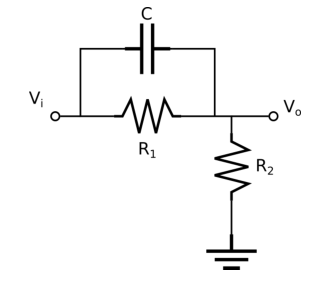
\includegraphics[width= 30mm]{fig3_1.png}\\
       \end{tabular}
\end{table}

\end{landscape}
%%%%%%%%%%%%%%
\end{document}
%%%%%%%%%%%%%%

%%%%%%%%%%%%%%%%%%%%%%%%%%%%%%%%%%%%%%%%%%%%%%%%%
% copyleft | Fabián Abarca Calderón, diciembre 2011
% Se autoriza su uso, modificación y reproducción
